\setchapterpreamble[u]{\margintoc}
\chapter{Controlli non distruttivi}
\labch{cap3}

\section{Introduzione}

I metodi roentgenografici appartengono alla grande famiglia dei \textbf{controlli non distruttivi} (CND).\\
Esiste un parallelismo fra corpo umano e materiali metallici: molte tipologie di analisi che vengono effettuate sul corpo umano possono essere fatte anche sui materiali metallici.

Soprattutto in ambito aerospaziale, il livello di sicurezza deve essere molto alto: si analizza il 100\% dei componenti e non un certo numero di pezzi a campione, per cui i controlli sono tutti di tipo non distruttivo. Tali controlli da un lato sono utili ad attestare la qualità del prodotto, cioè assicurare che il componente sia privo di difetti, dall’altro aiutano a migliorare la qualità e la produzione: si possono trovare metodi più economici e sicuri per produrre un pezzo.

\index{controlli non distruttivi}Le prove non distruttive (PND) consistono, per definizione, in quelle metodologie di indagine atte alla ricerca di \textbf{discontinuità} (failure) in un pezzo, senza distruggerlo o danneggiarlo, permettendone così il riutilizzo. Una failure rappresenta un malfunzionamento generale del componente, che non causa, per forza, la rottura. Tuttavia, il difetto non va sempre considerato come negativo, ma ha anche con un’accezione positiva, ad esempio nel caso di vacanze o dislocazioni, che sono fondamentali per i le proprietà dei materiali metallici.

Le PND hanno lo scopo di consentire l’emissione di giudizi di accettabilità dei singoli pezzi. La possibilità di estendere il controllo a tutti i componenti in una determinata costruzione consente di prevenire incidenti e disgrazie.

\section{Scelta di tipo di controllo}

Ogni tipo di controllo serve a vedere una certa tipologia di difetti, cioè i controlli non sono intercambiabili, ma sono spesso sovrapponibili.

La scelta del tipo di controllo da effettuare su un pezzo dipende da svariati fattori, i principali dei quali sono:
\begin{enumerate}
    \item \textbf{Tipologia di discontinuità} attesa:
    \begin{itemize}
        \item forma;
        \item posizione: se il difetto è superficiale si utilizza un metodo ottico-visivo, se è interno usano i raggi X;
        \item orientamento.\\
        Non esistono quindi metodi universali
    \end{itemize}
    \item \textbf{Limiti del metodo}: ogni metodo ha dei limiti intrinseci che ne circoscrivono il campo di applicabilità. Ad esempio, i metodi magnetici si posso applicare solo ai materiali ferromagnetici oppure per la ricerca di un difetto nel cuore di un pezzo di elevate dimensioni non si possono usare i raggi X, ma si opta per gli ultrasuoni;
    \item \textbf{Condizioni operative}: alcuni controlli richiedono una sorgente di forza motrice. Ad esempio, la radiografia richiede l’accessibilità del pezzo da ambo i lati, per posizionare sorgente di radiazione e pellicola, e questo non sempre è possibile, e i prezzi per le apparecchiature sono elevati;
    \item \textbf{Materiale del componente da controllare}:
    \begin{itemize}
        \item composizione chimica;
        \item caratteristiche meccaniche;
        \item trattamenti termici;
        \item rivestimenti superficiali.
    \end{itemize}
    \item \textbf{Dimensioni e spessore}: è importante valutare se il pezzo sia trasportabile o meno;
    \item \textbf{Complessità geometrica del componente}: quando si esamina un pezzo di grosse dimensioni non si può esaminare il 100\% della superficie, bensì si esamina un campione di struttura. Esso non può essere prelevato dall’interno del reperto, altrimenti si causerebbe la rottura: si è costretti ad utilizzare la superficie esterna. Tuttavia, nei materiali metallici esaminare un punto non è equivalente ad esaminarne un altro, poiché ciascuno ha caratteristiche diverse: bisogna scegliere attentamente la zona da analizzare, in modo che sia il più possibile rappresentativa dell’intero componente. Inoltre, spesso i reperti da analizzare presentano pareti e superfici più sottili o più spesse, che rendono difficile la scelta del campione.
\end{enumerate}

\section{Difettologia}\index{difettologia}\index{discontinuità}

Per discontinuità si deve intendere una soluzione di non continuità di un manufatto, che non pregiudica necessariamente l’utilizzo del manufatto stesso: infatti, solo dopo che la discontinuità è stata valutata sulla base di un criterio di accettabilità si può dire se vi è un difetto o meno.

Uno dei fattori di cui si deve tener conto quando si progetta una procedura d’esame è proprio il tipo di discontinuità che si pensa di dover rilevare.\\
Possono dividersi in:
\begin{itemize}
    \item bidimenisonali;
    \item tridimensionali;
    ed in
    \item superficiali;
    \item subsuperficiali.
\end{itemize}


Possono essere suddivise in cinque gruppi più un ulteriore gruppo per le discontinuità in esercizio:
\begin{enumerate}
    \item \textbf{Discontinuità congenite nel materiale}:
    \begin{itemize}
        \item \textbf{Ossidi}\index{ossidi}: essi derivano dalla reazione dell’ossigeno con elementi ossidabili ed influenzano la lavorabilità a caldo del materiale. Con la fucinatura vengono deformati e/o spezzettati secondo la deformazione principale. Non essendo materiali metallici, gli ossidi rappresentano una discontinuità nel materiale e formano dei buchi nel materiali di forma tondeggiante. La formazione di ossidi si può verificare dopo trattamenti termici come la saldatura;
        \item \textbf{Solfuri}\index{solfuri}: nascono dalla reazione dello zolfo con il ferro o con il manganese, sono molto plastici e seguono la deformazione del materiale. A differenza degli ossidi hanno una forma più allungata e sono delle discontinuità che indeboliscono il materiale. Il solfuro di ferro forma con il ferro un eutettico a 900°C, che impedisce la fusione del materiale. Tuttavia, negli acciai automatici, lo zolfo viene aggiunto intenzionalmente per facilitarne la lavorabilità alle macchine utensili;
        \item \textbf{Fiocchi}\index{fiocchi}: sono dovuti alla presenza di \textbf{idrogeno} disciolto nell’acciaio, che tende a riunirsi in “sacche” dove la pressione raggiunge valori elevatissimi e provoca delle lacerazioni del materiale. La sezione di un fiocco è puntiforme e i puntini rappresentano le bolle di idrogeno: essi si vedono solo quando il pezzo si rompe o se sono presenti in superficie;
        \item \textbf{Inclusioni metalliche e non metalliche\index{inclusioni}}: le più comuni inclusioni non metalliche sono quelle di silice di allumina, mentre quelle metalliche sono costituite da stagno e rame in quanto presenti nel materiale di presenza. Rame e stagno non si sciolgono nel ferro e formano con esso un eutettico basso-fondente e una fase a sé stante. Infatti, l’acciaio si ricava sia a partire dal minerali, negli altoforni, sia nelle acciaierie elettriche, a partire da rottami (automobili, lavatrici, elettrodomestici, etc) che vengono rifusi. Il rame deriva da cavi elettrici contenuti in ogni apparecchiatura, il piombo dalle batterie e lo stagno dalla brasatura dei cavi elettrici. Nei rottami, solo i vetri sono riciclabili al 100\%; gli pneumatici vengono rigenerati per non essere bruciati. Il piombo, lo stagno e il rame sono i principali inquinanti dell’acciaio. L’acciaio ricavato dalle acciaierie elettriche, quindi dai rottami, deve essere supportato dall’introduzione di acciaio puro, prodotto da acciaierie a ciclo integrale che lo producono a partire dal minerale (Ilva, Taranto). Per gli acciai ad elevato valore aggiunto, ad esempio gli acciai inox, le acciaierie acquistano i rottami di manufatti prodotti con i loro acciai, per essere sicuri della purezza del materiale.
    \end{itemize}
    \item \textbf{Discontinuità che insorgono durante la colata}:
    \begin{itemize}
        \item \textbf{Discontinuità di cristallizzazione}\index{discontinuità di cristallizzazione}: l’acciaio colato nella lingottiera o nella forma inizia la solidificazione dalle parti più esterne e con velocità di raffreddamento diverse tra le parti esterne e quelle interne, dando origine al dendritismo\index{dendrite}. Un dendrite è una forma morfologica di accrescimento di un grano in una struttura a “palizzata”, con cristalli molto grandi che si allungano perpendicolarmente all’asse e che si dispongono dall’esterno verso l’interno, seguendo il gradiente di temperatura. Al centro del materiale, vi sono cristalli più regolari di forma poligonale. Si hanno, quindi, proprietà differenti in base alle zone. Le impurità si concentrano nel liquido e si spostano man mano che il materiale si raffredda: la superficie esterna sarà di acciaio puro, mentre il cuore che raffredda per ultimo sarà un concentrato di impurità, che vengono trascinate dal liquido. Ciò causa una disomogeneità della struttura del materiale. I dendriti sono in parte eliminabili con le successive lavorazioni a caldo, attraverso ad esempio la ricottura dei lingotti. A causa della non uniformità del raffreddamento, poiché si raffredda prima la superficie esterna e successivamente il cuore interno, compaiono tensioni residue all’interno del materiale. Se un dendrite si spezza durante la laminazione, si possono spaccare perfino i rulli di laminazione a causa del contraccolpo della rottura;
        \item \textbf{Cavità di ritiro}\index{cavità di ritiro}: ono dovute alla contrazione del materiale, che si ha nella fase solidificazione (6\% per l’acciaio). Tale contrazione può dare origine a cavità nella parte che solidifica per ultima;
        \item \textbf{inclusioni}: parti di refrattario che si staccano dalla siviera (il contenitore dell’acciaio liquido), dal canale di colata o da altre attrezzature. Durante la solidificazione tendono a concentrarsi nella parte alta del getto (materozza): con una corretta eliminazione di quest’ultima, è probabile una loro eliminazione;
        \item \textbf{Cricche}: si formano a causa di parametri di colata sbagliati o ad errori di procedimento o di geometria (forti cambiamenti di spessore nel getto);
        \item \textbf{Porosità}: è spesso causata da gas di varia natura che rimangono intrappolati nel getto ed è strettamente legata alla tecnologia di produzione utilizzata. Infatti, nei gas come l’idrogeno, la solubilità diminuisce al diminuire della temperatura, quindi rimangono intrappolati nel materiale, creando dei pori che lo indoboliscono;
    \end{itemize}
    \item \textbf{Discontinuità che insorgono nei materiali durante l'esercizio}\index{fatica}: sono essenzialmente dovute alla fatica, cioè quando si ha un’applicazione di un carico variabile nel tempo. Facendo dei cicli di carico si formano delle microcavità superficiali che portano a lungo andare alla rottura del pezzo. Il 90\% delle rotture in esercizio è dovuta a fatica. La rottura da fatica dal punto di vista morfologico è divisa in tre zone:
    \begin{itemize}
        \item \textbf{zona d'innesco} del fenomeno, solitamente in prossimità di un poro o di una cricca, cioè di zone soggette a sforzi maggiori;
        \item \textbf{zona di propagazione}, dove la cricca si propaga a causa di cicli di carico e scarico;
        \item \textbf{zone di cedimento}, cioè la zona in cui si ha la cessione di scatto.
    \end{itemize}
    \item \textbf{Discontinuità dovute alle lavorazioni a caldo}, come lo strappo da fucinature e la ripiegatura;
    \item \textbf{Discontinuità da trattamento termico}: sono di tipo superficiale e possono essere causate da non corretta esecuzione del trattamento termico o anche da problemi legati alla geometria del pezzo;
    \item \textbf{Discontinuità nelle lamiere}: si possono avere paglie, cricche da tensioni, bugne, impronte, sdoppiature, inclusioni e segregazioni;
    \item \textbf{Discontinuità da saldatura}\index{discontinuità da saldatura}: le saldature uniscono due o più pareti solide realizzando la continuità del materiale. In tutti i casi in cui continuità risulti imperfetta si può parlare di discontinuità di saldatura. Le discontinuità possono trovarsi nella zona fusa (se si trovano qui significa che l’operazione saldatura non è stata eseguita bene) o nella ZTA. In questo caso si possono avere cricche a freddo o caldo, strappi lamellari e inclusioni solide (di scorie e di tungsteno) o gassose (porosità e tarli). Vi possono anche essere difetti dovuti all’eccesso di sovrametallo, ad un cordone d’angolo troppo convesso, a incisioni marginali, allo slivellamento dei lembi o alle irregolarità superficiali.
\end{enumerate}

\section{Metodo radiografico}\index{raggi X}

I raggi X (onde elettromagnetiche) sono prodotti entro un tubo radiogeno (tubo di Coolidge) per franamento degli elettroni accelerati ad alta velocità contro un anticatodo di tungsteno; alla finestra di uscita essi sono costituiti da uno spettro di radiazione di radiazione distribuito su varie lunghezze d’onda con valore minimo parti a $\lambda_{min}$=1,2395/kV, dove al denominatore compare il valore della tensione acceleratrice degli elettroni, generalmente alta.

E’ il metodo ideale per la ricerca di \textbf{difetti e discontinuità tridimensionali}: basa il suo principio sulla variazione di attenuazione che subisce una radiazione ionizzante attraverso la materia, quando i raggi X incidono su di un apposito convertitore (pellicola radiografica, schermo fluorescente, etc.) e riproducono l’immagine in chiaro-scuro dell’oggetto che hanno attraversato.

Presenta molti \textbf{vantaggi}:
\begin{itemize}
    \item applicabilità alla maggior parte dei materiali (no ferromagnetici);
    \item possibilità di rilevamento di difetti a profondità maggiore rispetto ad altri metodi; per difetti più
interni si utilizzano gli ultrasuoni;
\end{itemize}

ma anche \textbf{svantaggi}:
\begin{itemize}
    \item i difetti bidimensionali come le cricche possono essere rilevati se il loro orientamento rispetto all’asse della radiazione è parallelo;
    \item l’utilizzo della radiazione ionizzante richiede il rispetto di severe legge con conseguente aumento dei costi;
\end{itemize}

L’uso dei raggi $\gamma$\index{raggi $\gamma$} crea maggiori problemi a causa dell’impossibilità di spegnere la fonte: tali raggi derivano, infatti, dal decadimento radioattivo di particolari elementi ed è un processo naturale.

\section{Magnetoscopia}\index{magnetoscopia}\index{ferromagnetismo}\index{paramagnetismo}\index{diamagnetismo}

La maggior parte dei materiali metallici sono costituiti da acciaio nella configurazione ferritica $\alpha$. In questa condizione, il ferro è ferromagnetico, anche se non lo è sempre: se la temperatura è più alta della temperatura di Curie\index{temperatura di Curie} il materiale diventa paramagnetico, mentre al di sotto è ferromagnetico. Per il ferro, la temperatura di Curie è è pari a 768°C. I materiali ferromagnetici industrialmente utilizzabili sono essenzialmente tre: nichel, con punto di Curie a 345°C, cobalto a 1115°C e ferro come detto a 768°C. Per gli altri materiali metallici, il punto di Curie si trova al di sotto della temperatura ambiente ed è sconveniente dal punto di vista industriale perché questo implica dei dispositivi di raffreddamento.\\
La configurazione del ferro $\beta$\index{ferrite $\beta$} è quella CCC paramagnetica ed è presente fra i 768°C e i 1400°C. Si parla però sempre di ferrite $\alpha$ (presente fino a 907°C), di ferro $\gamma$ (presente con temperature comprese fra i 907°C e i 1400°C) e di austenite $\delta$ (presente con temperature superiori ai 1400°C) perché oltre il comportamento magnetico, non c’è nessuna differenza tra ferro $\alpha$ e $\beta$, a meno che non ci siano delle applicazione di tipo magnetico, come nel caso della magnetoscopia, che richiede ferro ferromagnetico.

Il comportamento della materia può essere ferromagnetico, paramagnetico e diamagnetico:
\begin{itemize}
    \item se il campo magnetico esterno viene aumentato di molto, il materiale è ferromagnetico;
    \item se il campo viene diminuito di poco, il materiale è diamagnetico;
    \item se il campo è aumentato di poco, è paramagnetico.
\end{itemize}

Se si introduce un materiale fatto in acciaio ferritico in una zona dove vi è un campo magnetico esterno, le linee di campo attraversano il pezzo, se esso è integro. Invece, se vi sono delle discontinuità le linee di campo vengono alterate.

La magnetoscopia consiste nel magnetizzare il particolare da esaminare in direzione appropriata e ad un dato livello di induzione, in modo da generare
un campo magnetico disperso in corrispondenza della discontinuità. Irrorando la superficie con un liquido vettore contenente in disperazione una fine polvere con caratteristiche ferromagnetiche, il campo magnetico disperso attrae tale polvere formando in corrispondenza delle discontinuità un accumulo (indicazione) osservabile ad occhio nudo, cioè le linee di campo divergono in presenza di un difetto. Questo metodo è idoneo per rilevare discontinuità superficiali e sub-superficiali ed è applicabile soltanto ai materiali ferromagnetici: acciai e ghisa, ad esclusione degli acciai inossidabili austenitici. 
\begin{marginfigure}[-4cm]
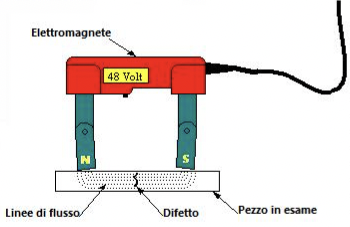
\includegraphics{images/img14.png}
\caption{Schema di contollo magnetoscopico}
\labfig{img14}
\end{marginfigure}

Questo metodo ha dei \textbf{vantaggi}:
\begin{itemize}
    \item è adatto a rilevare discontinuità superficiali e sub-superficiali;
    \item possibilità di parziale automazione con l’uso dei lettori ottici;
\end{itemize}

e come \textbf{svantaggi}:
\begin{itemize}
    \item applicabilità ai soli materiali ferromagnetici;
    \item l’esame è normalmente limitato alle zone accessibili;
    \item se il materiale è magneticamente duro, esso rimane magnetizzato e si forma una calamita. Esso deve essere smagnetizzato prima di essere utilizzato perché potrebbe causare interferenze con il resto della struttura.
\end{itemize}

\section{Liquidi penetranti}\index{liquidi penertanti}

Rappresenta una tecnica a metà tra un esame visivo e un esame strumentale, e si possono vedere solo difetti superficiali.\\
Il particolare da analizzare è immerso in un liquido a bassa tensione superficiale, capace di penetrare entro eventuali discontinuità affioranti in superfici.\\
Dopo un opportuno tempo di immersione il particolare viene estratto dal liquido e lasciato drenare. Mediante lavaggio viene asportato l’eccesso di penetrante e quindi si procede all’asciugatura in forno a circolazione di aria calda. Le discontinuità eventualmente presenti, a questo punto, contengono ancora del residuo di penetrante e se cosparse da un opportuno rilevatore, per adsorbimento si formano, sulla superficie del particolare, delle indicazioni più facilmente osservabili ad occhio nudo.
\begin{figure}[hb]
    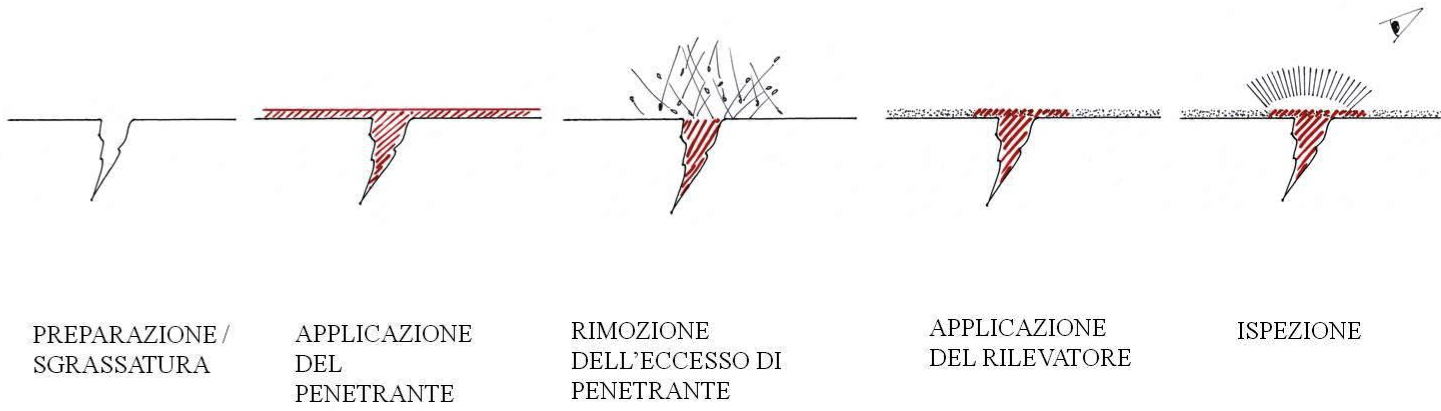
\includegraphics[width=0.9\textwidth]{images/img15.png}
    \caption{Processo di controllo tramite un liquido penetrante}
    \labfig{img15}
\end{figure}

Si tratta di un metodo idoneo a rilevare solo discontinuità superficiali ed è applicabile a qualunque materiale, purché non poroso (non va bene per materiali sinterizzati).

Ha come \textbf{vantaggi}:
\begin{itemize}
    \item applicabilità ad ogni tipo di materiale purché non poroso;
    \item semplice da eseguire;
    \item buona redditività;
    \item basso costo;
\end{itemize}

e come \textbf{svantaggi}:
\begin{itemize}
    \item non rileva discontinuità sotto pelle;
    \item solo in zone accessibili;
    \item nel caso di asportazione del liquido penetrante in eccesso con lavaggio in acqua, necessita il trattamento delle acque reflue.
\end{itemize}

\section{Ultrasuoni}\index{ultrasuoni}

Analoga analisi nel corpo umano: ecografia.
Si usano onde di tipo sonoro, cioè non onde ionizzanti, ma vibranti. Vi è un generatore di onde sonore che penetrano nel materiale e vengono respinte o smorzate se incontrano un difetto.

Vi sono due metodi: a \textbf{trasmissione}, in cui l’onda viene inviata e c’è un rilevatore che riceve le onde trasmesse dal materiale, e a riflessione, in cui l’onda torna indietro.

Gli ultrasuoni sono un metodo relativamente economiche e l’apparecchio può essere facilmente trasportato. Inoltre, è molto preciso ed è l’unico metodo che può penetrare molto in profondità.

Gli ultrasuoni sono onde elastiche ad alta frequenza (16000-20000Hz) e basano il loro principio sulla riflessione che un’onda acustica subisce quando, viaggiando all’interno di un mezzo, incontra un ostacolo alla sua propagazione.\\
Se l’ostacolo è posto normalmente alla direzione di incidenza dell’onda, questa ritorna verso la sorgente che l’ha generata.

Questo metodo nelle due applicazioni, a secco ed in immersione, risulta idoneo per la ricerca di discontinuità sia superficiali e sub-superficiali; viene inoltre impiegato nel controllo della sferoidizzazione delle ghise e per le misurazioni degli spessori (con precisione nell’ordine di 0,001mm). Se vi è un difetto vi saranno degli echi di difetto leggibili in un grafico.

I \textbf{vantaggi} sono:
\begin{itemize}
    \item velocità di esecuzione dell'esame;
    \item elevato livello di sensibilità;
    \item possibilità di rilevare difetti in profondità (fino a 20 m), poiché le onde acustiche si propagano nel mezzo, a differenza dei raggi X che si propagano nel vuoto;
    \item possibilità di automatizzare il controllo;
\end{itemize}

\textbf{Svantaggi}:
\begin{itemize}
    \item difficoltà di controllo dei materiali ad alta attenuazione acustica, cioè i materiali fonoassorbenti, come quiet steel e quiet alluminum, cioè materiali utilizzati per la riduzione del rumore;
    \item difficoltà dei pezzi a geometria complessa e ad elevata rugosità;
    \item sensibilità d’esame condizionata dallo stato della superficie del pezzo;
    \item impiego di personale molto specializzato per la lettura dei risultati.
\end{itemize}

Un altro metodo che sfrutta i principi magnetici ed elettrici sono le \textbf{correnti indotte}: avvolgendo il pezzo con un solenoide percorso da corrente, si genera un campo magnetico che induce delle correnti parassite nel pezzo. Se vi sono discontinuità, vi saranno delle alterazioni nella corrente indotta.

\section{Metodo ottico - Microscopia}\index{microscopia}

Sono analisi che si possono effettuare attraverso gli occhi. Se vi sono analisi che pretendono ricercare difetti non visibili ad occhio nudo, si passa alla microscopia per studiare la superficie. Quando si utilizzano metodi microscopici, deve essere scelto e preparato il campione. Una volta preparato, il campione viene inglobato per non essere alterato ed infine, lappato.